%%%%%%%%%%
%\subsection{Origin in general relativity}
%\textcolor{red}{Derive wave equation from einstein equation}\\

%%%%%%%%%%
\subsection{Heuristic introduction to gravitational waves}
\textcolor{blue}{A etoffer/compléter}
\vspace{1cm}\\
% origin
First detected in september 2015, gravitational waves were predicted by the theory of general relativity since 1916.
A relatively easy way of making them arise from general relativity is when considering an expansion around flat space-time by introducing a small perturbation in the metric.
A few computations and coordinate changes yield a wave equation for the metric.
Gravitational waves are, in general relativty, the analog of electromagnetic waves in electrodynamics but their nature differ greatly.
In the case of gravitational waves the curvature of space-time itself is following a wave equation, the waves can be seen as ripples in the curvature of space-time.
This implies that gravitational waves propagate through matter without being altered, although they can be altered by strong gravitational fields created by heavy objects.
Another notable result is that the gravitational waves propagate at the speed of light in vacuum.

% effects
What are the effects of gravitational waves ?
\textcolor{red}{Although propagating through space-time they only affect the space components of the metric, at first order.}
Two particles separated in space only in the direction of propagation of the wave will not see any effect, both their separation and proper separation will remain unchanged: the wave is purely transverse.
Other particles separated along directions tranverse to the direcion of propagation of the wave will have their proper separation oscillating proportionnaly to their separation, the intensity of the wave and following its frequency.

% transition to sources
The next interrogation is about the sources of gravitational waves.
Following-up on the analogy with electrodynamics where accelerating charged particles create electromagnetic waves, we can expect accelerating masses to produce gravitational waves.


%%%%%%%%%%
\subsection{Astrophysical sources overview}
\label{sec:sources}
%
The very first detection of gravitational waves was identified as what is called Compact Binary Coalescence (CBC) meaning the coalescence of two compact objects.
In the case of the first detection called GW150914 the properties of the source led to the conclusion that the two objects were black holes, we then talk about Binary Black Hole systems or BBH.
Aside from the fusion of black-holes there were also expectations regarding Neutron Star-Black Hole (NSBH) and Binary Neutron Star (BNS) coalescing systems emitting detectable gravitational waves.
The first BNS detection occured in August 2017 and we had to wait until 2020 for the first detections of NSBH.
The coalescence process of a CBC is usually described in two to three steps:
\begin{itemize}

\item Inspiral: the two objects are rotating around each other at high speed.
  They get closer as time goes and their speed increases, reaching values of the order of magnitude of the speed of light in vacuum.
  Gravitational waves are emitted throughout the full duration of the process.
  The frequency and intensity of the waves increase as the object get closer and faster.
  
\item Merger: the two objects have become so close that they reached their innermost stable circular orbit (ISCO) and merge extremely rapidly.
  %% donner formule R_isco ?
  The gravitational wave signal reaches its maximum intensity and frequency at this point.
  What remains after the merger depends on the initial system.
  In the case of a BBH the resulting object will be a more massive blackhole.
  In a NSBH system the black hole will end up disrupting and absorbing the neutron star thus yielding in the end a black hole.
  Several scenarii can happen when dealing with a BNS system: the final object can either be a black hole or a neutron star.
  If it is a neutron star it may or may not collapse into a black hole. The collapse can in turn occur in a matter of seconds or over a longer duration.
  All of it depends on the properties of the two neutron stars and of the resulting object.
  
\item Ringdown: This step is only relevant if the resulting object is a blackhole.
  After the merger the black hole is in an excited state and is possibly very asymetric.
  It will radiate energy through gravitational waves until it reaches equilibrium.

\end{itemize}

Figure \ref{fig:inspiral} shows a schematic view of the full process.
%
\begin{figure}
  \centering
  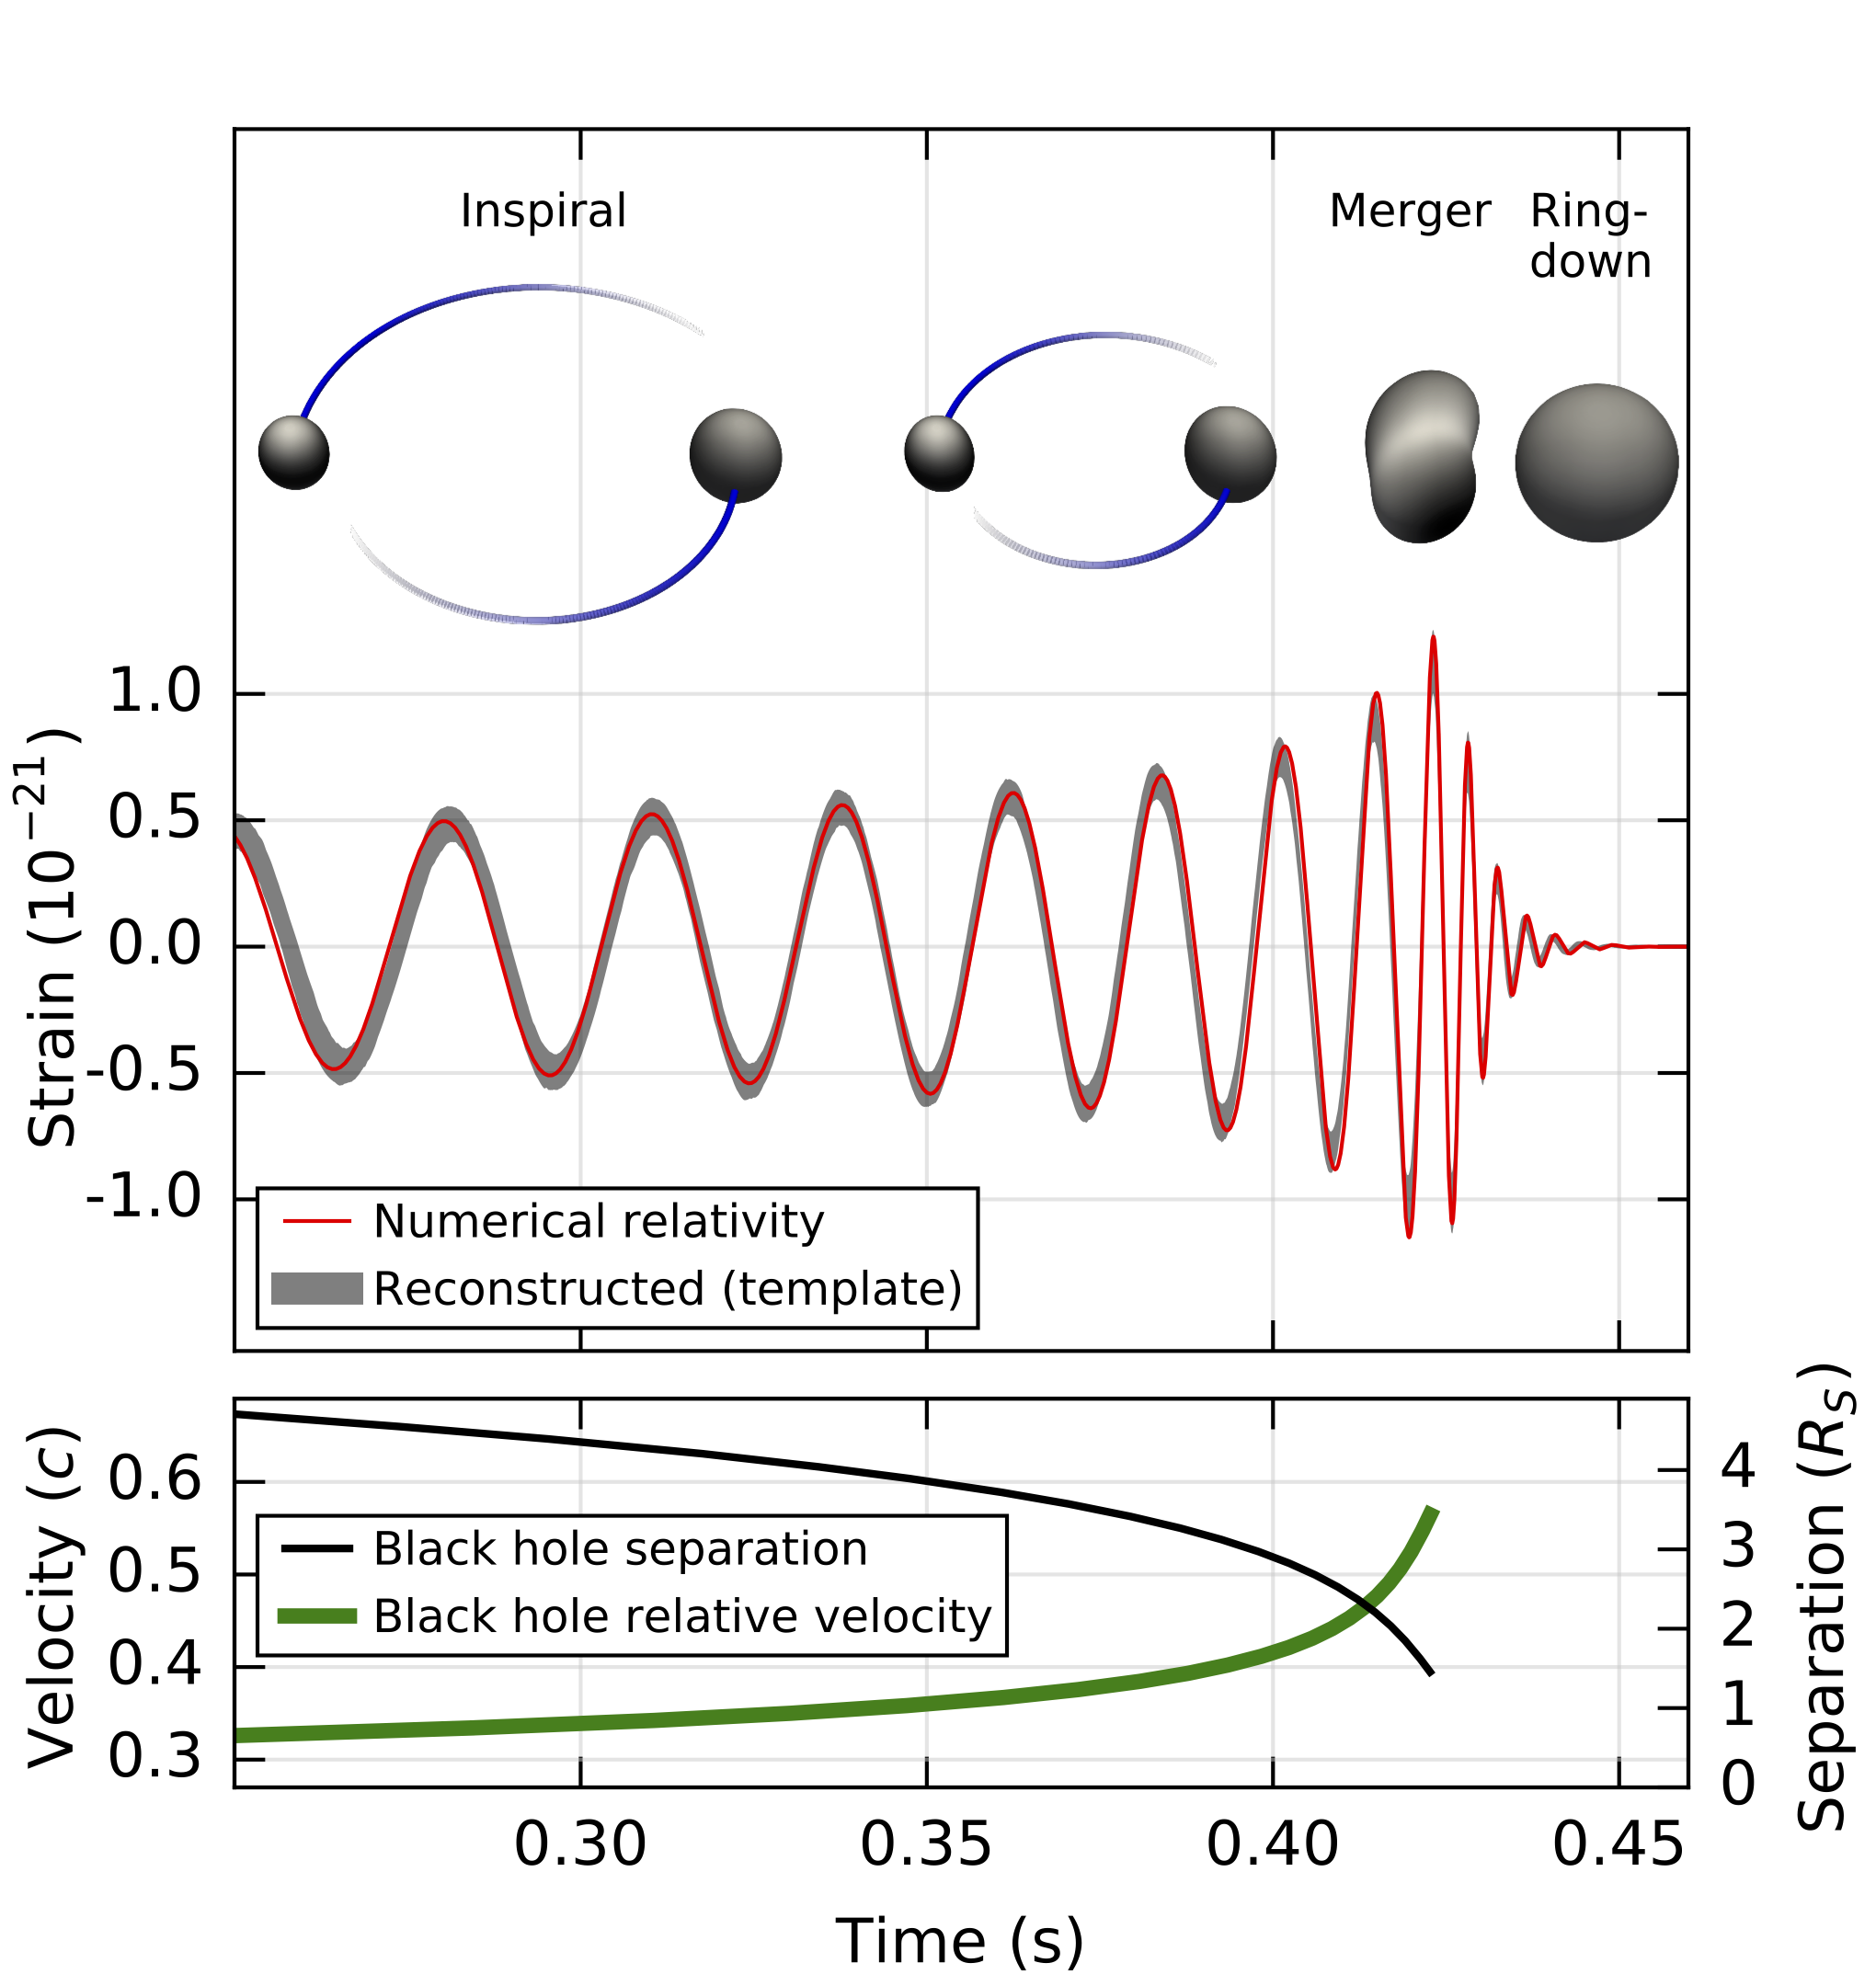
\includegraphics[width=0.5\linewidth]{sectionGW/inspiral.png}
  \caption{Figure taken from \cite{gw150914}. Top panel: schematic view of the inspiral and merger of two black holes with the evolution of the waveform over time. Bottom panel: evolution of the black hole separation and relative speed during the process.}
  \label{fig:inspiral}
\end{figure}
%

The LIGO-Virgo-Kagra collaboration also runs searches for other type of sources, among which we can cite the following:

\paragraph*{Search for lensed events}
Gravitational lensing is caused by massive object that distort space-time.
The effect of gravitational lensing is observed for electromagnetic waves, deflecting them and creating for the observer several images of the sources that can be magnified or distorted.
Gravitational waves should also be subject to gravitational lensing if the source, e.g. a compact binary merger, is located behind a massive object such as a galaxy cluster in which case we talk about ``massive lense'' and ``strong lensing'', or even a lower mass object such as a star or compact object yielding ``microlensing''.
Strong lensing is expected to create multiple signals that the observer detects as a repeated waveform since strong lensing should not change the frequency evolution of the waves \cite{LVK_lensing}.
Due to the repetition of the signal in detector data, lensed events should offer a better localization of the source than regular CBC events.
Microlensing may be seen by a beating pattern in the waveform as detailed in \cite{lensing_beating}.

\paragraph*{Search for continuous waves}
Continuous waves are gravitational waves emitted on a much longer time scale than those of CBC mergers.
Possible sources of such waves are rotating neutron stars with an asymmetry or non-uniformity causing a deformation.
The continuous waves emitted by such a system would have a frequency close to rotation frequency of the neutron star (or related to it) and would therefore be quasi-monochromatic following the spin-down of the star \cite{LVK_cw}.
Searches for continuous waves can be
\begin{itemize}
\item targeted, meaning that data are analyzed region of the sky where there is a known rotating neutron star,
\item directed, data of a specific region of the sky where there is no known source are analyzed,
\item all-sky, trying to find sources from all direction.
\end{itemize}

\paragraph*{Search for gravitational waves bursts}
Bursts are very short transients that can last from a few seconds to a few milliseconds .
Potential sources of gravitational waves bursts are core-collapse supernovae, neutro star excitations, cosmic strings \cite{LVK_burst}...
Burst searches can be either modelled searches as for CBC searches or unmodelled to identify excess of power in the detectors.

\paragraph*{Search for a stochastic background of gravitational waves}
The many sources of gravitational waves that we do not detect directly still emit gravitational waves that can reach us.
These unresolved sources are distributed across the whole sky.
The waves they create are expected to combine and create a stochastic background of gravitational waves \cite{stochastic}.
This background should be isotropic at first order but may have small fluctuations making it anisotropic as the cosmic microwave background \cite{cmb}.
Both type of searches exist \cite{LVK_stochastic_aniso,LVK_stochastic_iso}.

%%%%%%%%%%
\subsection{Properties of gravitational waves and their sources}

\textcolor{blue}{Texte incomplet}\\
The waveform of gravitational waves produced by a CBC is determined by the source properties namely the masses of the two objects and their spins.
We call by convention mass1, spin1 and write $m_1$, $s_1$ the mass and spin (orthogonal to the inspiral plan) of the heavier object and mass2, spin2 ($m_2$, $s_2$) the mass and spin of the lighter one.
The spins are defined using the angular momentum $J_{1,2}$ of the two objects and normalized by the masses:
\begin{equation}
  s_i = \frac{J_i}{m^2_i} \text{  }, \text{  } i \in \{1,2\}
  \label{eq:spin}
\end{equation}
Their values can range from $-1$ to $1$.

Additionally we define five quantities, the total mass
%
\begin{equation}
  M_{\textrm{tot}} = m_1 + m_2
\end{equation}
%
the reduced mass
%
\begin{equation}
  \mu = \frac{m_1 m_2}{M_{\textrm{tot}}}
\end{equation}
%
the chirp mass
%
\begin{equation}
  \mathcal{M} = m_{chirp} = \frac{ \left( m_1m_2 \right)^{\frac{3}{5}} }{ \left( m_1 + m_2 \right)^{\frac{1}{5}} } = \mu^{3/5}M_{\textrm{tot}}^{2/5}
  \label{eq:mchirp}
\end{equation}
%
the mass ratio
%
\begin{equation}
  q=\frac{m_1}{m_2}
\end{equation}
%
and the effective spin
%
\begin{equation}
  \chi_{\textrm{eff}} = \frac{s_1m_1\cos t_1 + s_2m_2\cos t_2}{m_1 + m_2} \stackrel{\textrm{\tiny (anti)aligned spins}}{=} \frac{s_1 m_1 + s_2 m _2}{m_1 + m_2}
  \label{eq:spin_eff}
\end{equation}
%
with $t_1$ and $t_2$ the tilt angles of each object with respect to the orbital angular momentum of the binary system.

%
Gravitational waves can be written as a mixing of two polarizations that are \SI{45}{\degree} apart \cite{polarization} called the ``plus polarization'', $h_+$, and ``cross polarization'', $h_\times$, owing to the directions in which they stretch and squeeze space.
Figure \ref{fig:polarization} shows their effect on point particles.

These polarization can be written, for a CBC system in circular orbit, as \cite{Will_2014}:
%
\begin{equation}
  \begin{split}
    h_+ =& -\frac{2\mathcal{M}}{R} (2\pi \mathcal{M} f_b)^{2/3} (1+\cos^2 i) \cos(2\Phi_b (t))\\
    h_\times =& -\frac{2\mathcal{M}}{R} (2\pi \mathcal{M} f_b)^{2/3} (2\cos i) \sin(2\Phi_b (t))
  \end{split}
  \label{eq:polarization}
\end{equation}
%
Where $i$ is the inclination of the system with respect to the plane of the sky, $f_b$ is the orbital frequency of the binary, and $\Phi_b(t) = 2\pi \int^t f_b(t') dt'$ is the orbital phase.
$R$ is the characteristic scale for the distance to the system and can be taken as the luminosity distance
\begin{equation}
  D_L(z) = (1+z) \int_0^z \frac{dz'}{H(z')}
  \label{eq:luminosity_distance}
\end{equation}
where $z$ is the redshift, H is the Hubble factor such that $H = a^{-2} da/d\eta$ with $a(\eta)/a(\eta_0) = (1+z)^{-1}$ and $\eta$ the conformal time \cite{luminosity_distance}.
or the effective distance \cite{findchirp}
\begin{equation}
  D_{\textrm{eff}} = D \left( F_+^2 \left(\frac{1+\cos^2i}{2}\right)^2 +F_\times^2 \cos^2i \right)
  \label{eq:effective_distance}
\end{equation}
with $F_+$ and $F_\times$ are the interferometer antenna responses to the plus and cross polarization (shortly described in section \ref{section:detection}).

What we measure on earth are actually the redshifted quantity, such as the redshifted chirp mass $\mathcal{M}_z = (1+z) \mathcal{M}$ and redshifted frequency $f_z = f/(1+z)$.

% 
\begin{figure}
  \centering
  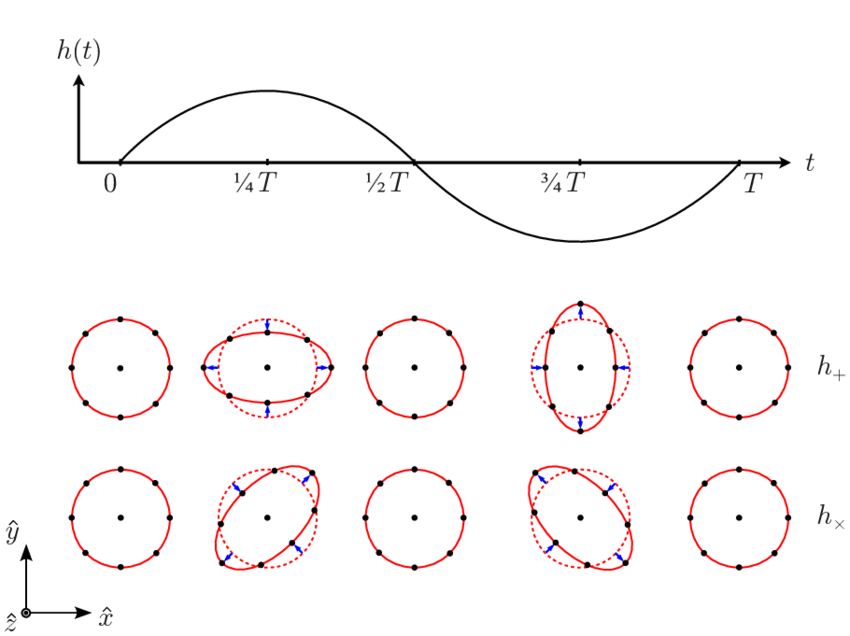
\includegraphics[width=0.5\linewidth]{sectionGW/polarization.png}
  \caption{Plot from \cite{polarization_novak}. Plus and cross polarization of a gravitational wave propagating along the z axis and their effect on a set of freely falling point-like particles.}
  \label{fig:polarization}
\end{figure}
%


\textcolor{red}{shape of the wave / chirp ?}\\

\textcolor{red}{faire plots de waveform pour différentes valeurs de mchirp et spin, anti-alignage des spins, pour differentes fréquences de départ}\\

\textcolor{red}{donner formule R isco, nu isco ?}

\begin{equation}
  \nu_{\text{isco}} = ....................................................
  \text{\textcolor{red}{attention doublon avec \ref{eq:f_isco} ?}}
  \label{eq:nu_isco}
\end{equation}

\begin{figure}
  \centering
  \begin{minipage}{0.45\linewidth}
    
\includegraphics[width=\linewidth]{placeholder.png}
    \caption{Plot plusieurs waveform pour différentes valeurs de chirp mass}
    \label{fig:waveform_mchirp}
  \end{minipage}
  \hfill
  %
  \begin{minipage}{0.45\linewidth}
    
\includegraphics[width=\linewidth]{placeholder.png}
    \caption{Plot plusieurs waveform pour différentes valeurs de spin effectif}
    \label{fig:waveform_spinEff}
  \end{minipage}
  \hfill
  %
  \begin{minipage}{0.45\linewidth}
    
\includegraphics[width=\linewidth]{placeholder.png}
    \caption{Plot plusieurs waveform pour spins alignés anti-alignés}
    \label{fig:waveform_spinAlign}
  \end{minipage}
  \hfill
  %
  \begin{minipage}{0.45\linewidth}
    
\includegraphics[width=\linewidth]{placeholder.png}
    \caption{Plot plusieurs waveform pour différentes valeurs de starting frequency}
    \label{fig:waveform_startFreq}
  \end{minipage}
  \hfill
\end{figure}



%%%%%%%%%%
\subsection{Motivations for detection}
\label{sec:motivations}
Aside from the undiscovered type of sources listed in section \ref{sec:sources} we present here other motivations for the detection of gravitational waves.

\paragraph*{Multi-messenger astronomy}
\label{sec:multimessenger}
The goal of multi-messenger astronomy is to better understand the population of astrophysical objects, the environement in which they evolve and uncover the origin of cosmic rays.
In the same way that different light frequencies give different informations, which has motivated the developpement of multi-wavelength astronomy, the addition of cosmic rays, high energy neutrinos and gravitational waves allows to gather even more information about the sources.
An overview of milestones and discoveries is given in \cite{multimessenger}.
There are a lot of efforts put into making joint observations of the different type of messengers.
Association between electromagnetic waves and high energy neutrino was reported by several observatories following the detection of neutrinos with a source localization compatible with a known $\gamma$-ray flaring blazar \cite{blazar_neutrino}.
The IceCube collaboration also reported evidence of an excess of neutrinos compatible with the localization of a nearby active galaxy \cite{agn_neutrino}.
A joint observation of gravitational waves and electromagnetic waves also occured with GW170817 \cite{gw170817}, the very first detection of a BNS merger which was followed up by a $\gamma$-ray burst.
Yet no joint observation of high energy neutrinos and gravitational waves was done to date \cite{hen_gw_antares,hen_gw_icecube} to form the missing link which would help us understand better CBC type events and the objects that form them.


\paragraph*{Tests of general relativity}
\label{sec:testingGR}
The list of tests given in this section is non-exhaustive and the reader is encouraged to read through the cited publications for more details.

\vspace{0.2cm}
\textbf{Propagation speed:} General relativity predicts that gravitational waves propagate non-dispersively at the speed of light in vaccuum.
Any deviation observed would be strong evidence in favor of alternative gravity models which predict some variations of the propagation speed.
This could come, for instance, from the coupling with lingering gravitational fields or if the propagation of gravitation is associated to a massive field which would imply a massive graviton \cite{Will_1998,Will_2014,testingGR}.
On the observational side of things, a straightforward way to test the propagation speed is to compare the arrival time of gravitational waves to the arrival time of electromagnetic waves for a given event although this requires precise knowledge on the emission times of both which is not yet the case.

\vspace{0.2cm}
\textbf{Polarizations:} Another test of general relativity is done by considering the polarization of gravitational waves.
General relativity allows for only two tensor polarization while many theories predict four more of different natures: two scalar polarization and two vector polarization, as shown by figure \ref{fig:other_polarization}.
These other polarizations are being searched for through continuous waves searches \cite{other_polarization_cw}, stochastic gravitational waves background searches \cite{polarization}, and using CBC events with prospects for searches using future detectors \cite{testingGR,other_polarization_cbc}.

\vspace{0.2cm}
\textbf{Deviation from waveforms predictions:} Waveforms are predicted by general relativity and used to look for signal in the detector output.
Deviations are being searched for by looking at the residual power when substracting the predicted waveform of a detected signal to the data.
A remaining excess of power would be an indicator of such deviation \cite{testingGR}.
%
\begin{figure}
  \centering
  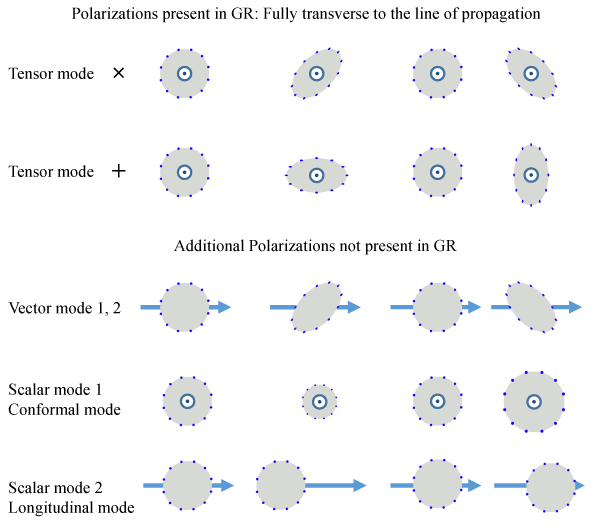
\includegraphics[width=0.6\linewidth]{sectionGW/other_polarization.png}
  \caption{Figure taken from \cite{other_polarization}. ``$+$'' and ``$\times$'' polarizations along other possible type of polarizations that are not predicted by general relativity.}
  \label{fig:other_polarization}
\end{figure}
%


\paragraph*{Measure of the Hubble constant}
\label{sec:H0}
The Hubble constant is measured by studying the distance versus redshift relationship of astrophysical populations of objects.
Systems which allow such measurement are called standard sirens.
It is possible to measure the luminosity distance (eq. \ref{eq:luminosity_distance}) of gravitational waves events but we still need an independent measurement of the redshift to properly establish the relationship of one versus the other.
GW170817 was by itself a standard siren thanks to the electromagnetic counterpart and allowed for a measurement of $H_0 = 70.0^{+12.0}_{-8.0}$ \SI{}{km.s^{-1}.Mpc^{-1}} \cite{H0_gw170817}.
For others we have to rely on the redshift measurement of a known host galaxy (or marginalizing over several possible host galaxies).
A refined analysis using this method yielded a value of $H_0 = 68.7^{+17.0}_{-8.3}$ \SI{}{km.s^{-1}.Mpc^{-1}} \cite{H0_LVK}.
The value of the Hubble constant has been a hot topic for decades now with measurements that are discrepant up to the $4-6\sigma$ level \cite{H0_1} as shown on figure \ref{fig:H0}.
Future measurements with better precision will allow to constrain even more the value of the Hubble constant for cosmological models.
%
\begin{figure}
  \centering
  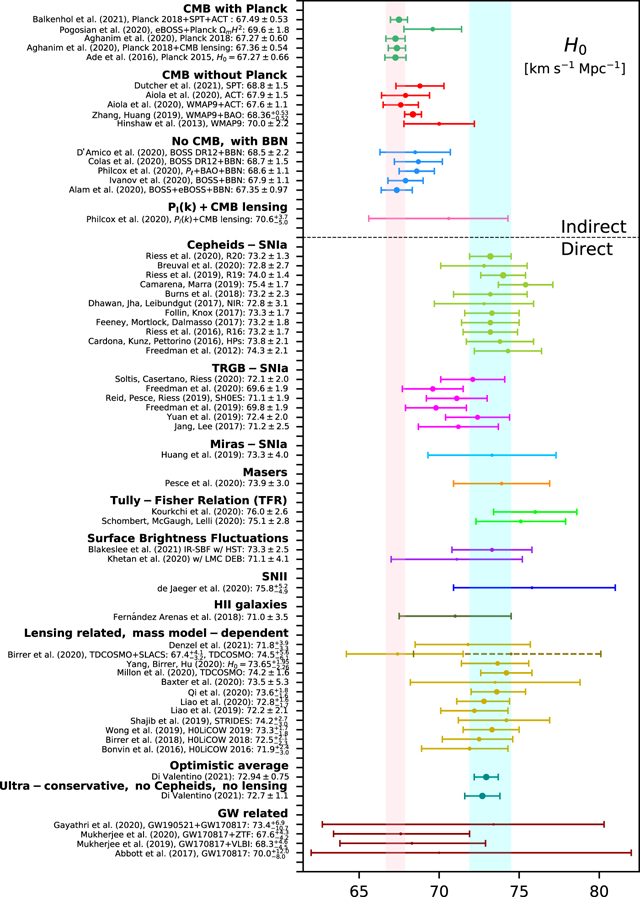
\includegraphics[width=0.7\linewidth]{sectionGW/measurementH0.jpg}
  \caption{Figure taken from \cite{H0_1}. Direct and indirect $H_0$ measurements 68\% CL intervals by various missions and collaborations. From \cite{H0_1}: ``The cyan vertical band corresponds to the H0 value from SH0ES Team \cite{shoes} (R20, $H0 = 73.2 \pm$ \SI{1.3}{km.s^{-1}.Mpc^{-1}} at 68\% CL) and the light pink
vertical band corresponds to the H0 value as reported by Planck 2018 team \cite{Planck_2018} within a $\Lambda$CDM scenario.''}
  \label{fig:H0}
\end{figure}
%

\paragraph*{Constraining the neutron star equation of state}
\label{sec:EOS}
The neutron star equation of state (EOS) relates state variables such as pressure and density and describes the nuclear matter at extremely high density inside the star.
It is used to derive many properties of a neutron star such as its radius, mass, moment of inertia, tidal deformability...
The EOS also allows, based on the neutron star masses and populations, to constrain the formation mechanisms of neutron stars.
Many efforts have been done to derive equations of state describing the neutron star matter from the crust to the inner core yet the EOS is widely unconstrained and different theoretical approach yield different equation of state \cite{EOS_Douchin_2001,EOS_Lattimer_2001}.
Gound-based experiment aiming at studying the nuclear matter at extremely low temperature and high density cannot reproduce the conditions inside a neutron star and we must therefore rely on astrophysical observations through (non-exhaustively) radio pulsars, X-ray binaries and more interestingly for us, gravitational waves emitted by BNS mergers \cite{EOS_gw170817,EOS_pulsar,EOS_Lattimer_2021}.
The tidal deformability caused by each neutron star of the binary on the other is the quantity that is best measured to constrain the EOS and is used to derive the radii of the two neutrons stars of the binary.
These measurement can also be combined with the mass measurement obtained from the detection of the BNS and can then be used to place constrains on the EOS.

\paragraph*{Rate et populations of CBC events}
\label{sec:rateNpop}
It is also possible to consider CBC events not as individual events but as a population of source to study some of their properties.
This is especially relevant with the coming of O4 where we expect many more detections.
Quantities that can be derived from such studies include the merger rate of CBC type events and their mass distribution.
Using the GWTC-3 catalog \cite{gwtc3} the merger rate were reported in \cite{rate_and_pop} to be between \SI{10}{Gpc^{-3}.yr^{-1}} and \SI{1700}{Gpc^{-3}.yr^{-1}} for BNS events, \SI{17.9}{Gpc^{-3}.yr^{-1}} and \SI{44}{Gpc^{-3}.yr^{-1}} for BBH events at redshift $z=0.2$ and between \SI{7.8}{Gpc^{-3}.yr^{-1}} and \SI{140}{Gpc^{-3}.yr^{-1}} for NSBH events.
They also report a uniform mass distribution for neutron stars ranging from $1.2^{+0.1}_{-0.2}$ \msun and $2.0^{+0.3}_{-0.3}$ \msun, a power law with peaks at $\mathcal{M}_{c} = 8.3^{+0.3}_{-0.5}$ \msun and $\mathcal{M}_{c} = 27.9^{+1.9}_{-1.8}$ for BBH mergers.

\paragraph*{Subsolar mass searches}
\label{sec:ssm}
The discovery of a subsolar mass CBC, i.e. a CBC with at least one component lighter than $1$ \msun, would be evidence for a new formation mechanism of compact object as current models of stellar evolution for massive stars only allow for a collapse into a neutron star or a black hole heavier than the sun \cite{ssm_O3a,ssm_O3b}.
Possible subsolar mass objects are primordial black holes \cite{primordial_bh} or black holes formed from the collapse of dark matter \cite{dm1,dm2,dm3} which would directly point towards new physics.
Subsolar mass searches are run by some CBC search pipelines with a dedicated parameter space.
MBTA is one of them.


\paragraph*{Search for exotic compact objects}
\label{sec:exotic}
Many exotic compact objects have been theorized but their existence remains to be proven.
The waveform of the coalescence of some of these objects is expected to be identical to the one of a BBH signal up to the merger or post-merger phase, while others may radiate gravitational waves by themselves or have some effect on gravitational waves such as lensing \cite{ECO1,ECO2}.
Examples of exotic compact objects are:
\begin{itemize}
\item Gravastars, introduced as an alternative solution to the final product of a gravitational collapse into a point-like object that is not a black hole \cite{gravastar1,gravastar2},
\item Wormholes theorized as space-time distortions that connect distant parts of the universe as a shortcut would \cite{wormhole2,wormhole1},
\item Boson stars, constructed from the association of a scalar field and gravity, they would consist of bosons stable or unstable that are held together by gravity \cite{boson_star},
\end{itemize}
One can also cite fuzzballs \cite{fuzzball}, firewalls \cite{firewall}, horizon-less black holes \cite{horizonless_bh}.



